\documentclass{ctexart}
\usepackage[top=1in,bottom=1in,left=1in,right=1in]{geometry}
\begin{document}
\section{偏心环的渗透计算}
先看同心环的情况,当内外环都是固定时,如下图。 \\
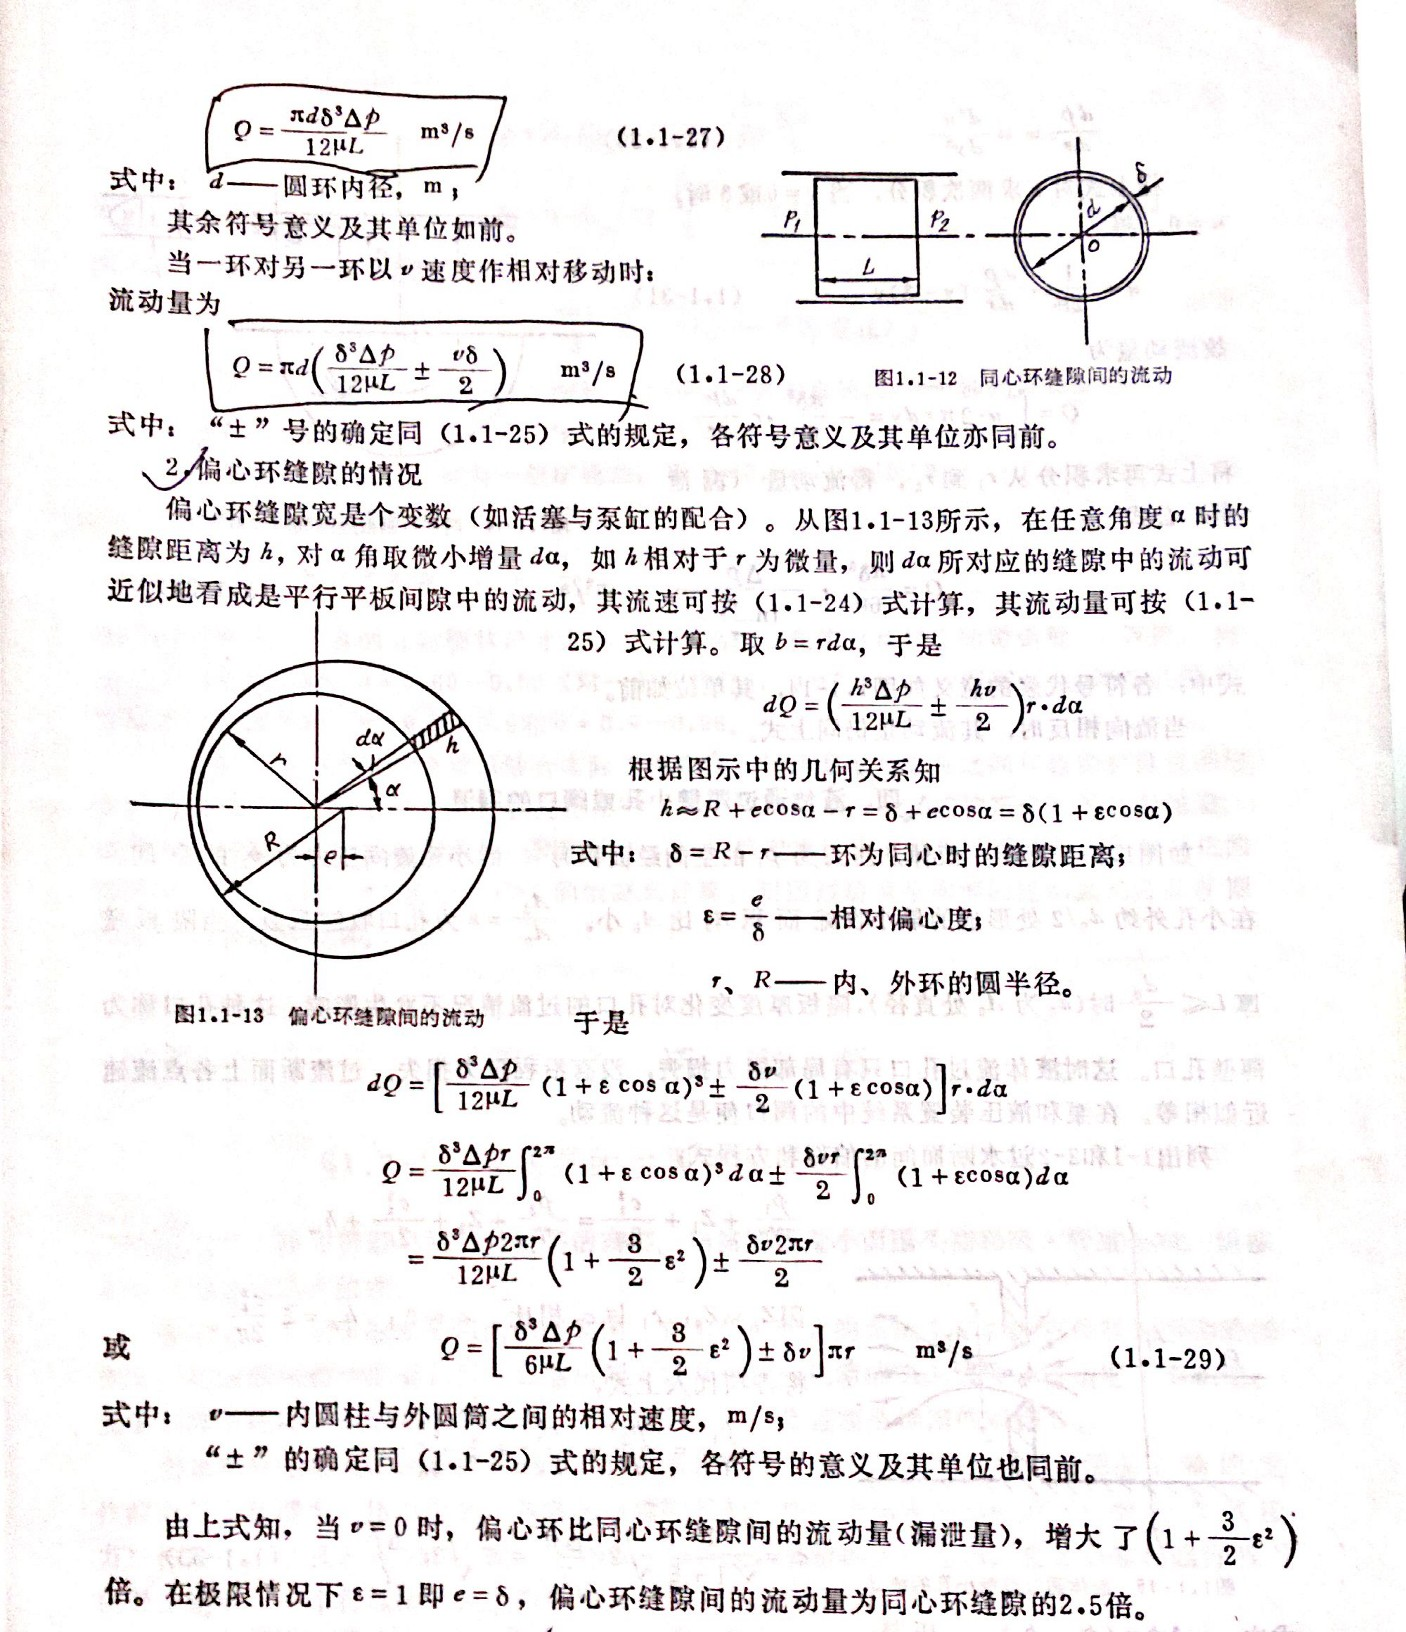
\includegraphics[width=\textwidth]{no1.jpg}
两环相对运动时,当v的方向与压差方向相反时,取``-"号;当其方向相同时,取``+"号。

\section{离心泵的设计思路}
\begin{enumerate}
	\item 结构形式的确定 
	\begin{enumerate}
		\item 离心泵设计流量和扬程一般是给定的。
		\item 泵吸入和排出口径由公式和查表确定。
		\item 结构形式的选择,包括原动机的选择、确定转速$ n $、比转数$ n_s $和级数$ i $、结构形式(单双吸、单双级、支承形式等)和轴径的计算。
	\end{enumerate}
	\item 叶轮设计(速度系数设计法)
	\begin{enumerate}
		\item 通过叶轮入口速度和通过叶轮的流量,根据公式确定叶轮入口直径$ D_0 $。
		\item 根据比转数和$ D_0 $确定叶片入口边直径$ D_1 $
		\item 根据公式确定叶片入口处绝对速度$ C_1 $、宽度$ b_1 $、圆周速度$ u_1 $、轴向速度$ C_m $,确定叶片数$ z $和叶片入口安放角$ \beta_1 $等
	\end{enumerate}
	\item 压出室和吸入室的设计
	\begin{enumerate}
		\item 压出室
		\item 螺旋形涡室的设计
		\item 吸入室的设计
	\end{enumerate}
	\item 径向力、轴向力的平衡
	\item 主要零部件的强度计算,包括叶轮强度计算、泵体强度计算、泵体密封面连接螺栓的计算等
	\item 离心泵主要通用零部件的选择,包括轴封结构的选择、轴承部件的选择、冷却系统的选择、联轴器的选择等
	\item 离心泵主要零部件的技术要求,包括过流部件的铸造偏差、泵轴叶轮泵体和总装配的技术要求
\end{enumerate}
\section{海水液压传动技术的优缺点}
海水液压传动技术的优点:
\begin{enumerate}
\item 传统的液压系统主要用矿物型液压油作介质,既浪费石油资源,又将产生泄漏、污染、易燃等一系列严重问题。不宜在高温、明火、矿井下等环境中工作,特别是对于存在有波浪、暗流等诸多不利因素的水下作业、 舰艇、 海洋开发、河道工程等。利用海水作为液压系统的工作介质,则可用于上述环境。
\item 无环境污染,无火灾危险。
\item 无购买、 运输、 贮存等问题, 既节约能源、 又降低了费用。
\item 可以不用回水管、不用水箱。液压系统大为简
化, 系统效率提高。
\item 可以不用冷却、 加热装置。
\item  海水温度稳定.介质粘度基本不变,系统性能稳定。
\item 海水粘度低,系统的沿程惯性小.
\end{enumerate}
海水液压传动技术的缺点:
\begin{enumerate}
	\item 与矿物型液压油相比,海水具有腐蚀性强、粘度低、润滑性差、汽化压力高等特点,原有的液压元件与海水完全不相适应,必须研制新型的海水液压元件。
	\item 海水的粘度大约只有液压油的$ 1/20\~{}1/40$,其润滑性差,运动摩擦副对偶面上很难形成液体润滑膜。很
容易产生边界摩擦或干摩擦,加之外界污染物如海水中的微细砂粒和内部磨屑的侵入,使得磨损加剧,摩擦损失增加,内部泄漏增大,容积效率降低,寿命缩短。特别是海水具有很强的腐蚀性,材料表面会发生复杂的物理化学反应,使之脆弱化,磨损会剥落受损的表层组织,内部高速液流带走磨屑后,使其迅速暴露出新鲜表面。新鲜表面又将受到上述作用剥落成磨屑,如此反复作用,材料的疲劳强度会太大下降,破坏重加严重。因此,改善元件的耐磨性、抗腐蚀性、抗疲劳持性是海水液压传动研究中必须首先解决的问题。
\item 海水的汽化压力比液压油高数千倍,加之系统中海水高速流动,很容易产生气蚀现象。气蚀不仅使振动和嵊声大为加剧,系统性能下降,而且还对材料具有严重的坏食作用。所以,必须分析气蚀产生的机理,提高系统的抗气蚀能力,延长系统寿命。	
\end{enumerate}
\section{热油锅炉的优点、原理}
\textbf{原理:}热油锅炉的介质是导热油,其工作原理和蒸汽锅炉一样。从热油循环泵开始,导热油进入废气锅炉,并在其中吸收废气热量(船舶在航行时),然后进入燃油辅锅炉,在此吸收燃油燃烧产生的热量。 温度升高了的热油从辅锅炉出来, 分几路进入相应的管路,去加热需要热量的系统或设备,并在这些系统或设备中放出热量后,返回到循环泵的吸入端。导热油在循环泵的驱动下不断的循环,在炉内加热后流到用户管道,然后通过密封的排气膨胀箱流回炉内重新加热。排气膨胀箱借助导热油体积的膨胀,把空气和蒸汽自动排放出系统,并在箱内把系统内导热油的温度降低到合理的程度,以防高温氧化。

\textbf{优点:}1.热媒油锅炉炉装置具有较高的热效率。热媒油锅炉内构造特殊,高温低压,加热温度均匀,热效率高,热媒油循环使用,除交换给热压机热量外没有任何热量外泄损失。2.热媒油锅炉的安全性高。热媒油在管路中流量所需压力,一般$0.4\~{}0.6Mpa$即可,属低压范围,对设备的耐压要求低,安全性好。3.热媒油锅炉易于实现自动控制,选择比例式或上下限温度控制器控制燃烧器即可满足温度控制要求。4.热媒油锅炉维护管理方便。

\textbf{缺点:}无论轻质油或热媒油,在流动时与管内壁的接触部分,流速较慢而液温较高,形成一种薄层,称为温度临界层,如果该临界层温度超过热媒油的最高允许温度,就会加速热媒油的劣化,进而产生高温物质而损伤管壁,需要精心设计,才能避免这方面的问题。一般说来,热媒油锅炉性能优越,燃烧完全,不会形成空气污染。但热媒油漏泄会对环境造成污染,废弃的热媒油需要进行处理以避免对环境的污染。这是使用热媒油锅炉需要引起重视的方面。
\section{空调制冷的计算}
\begin{figure}[!h]
	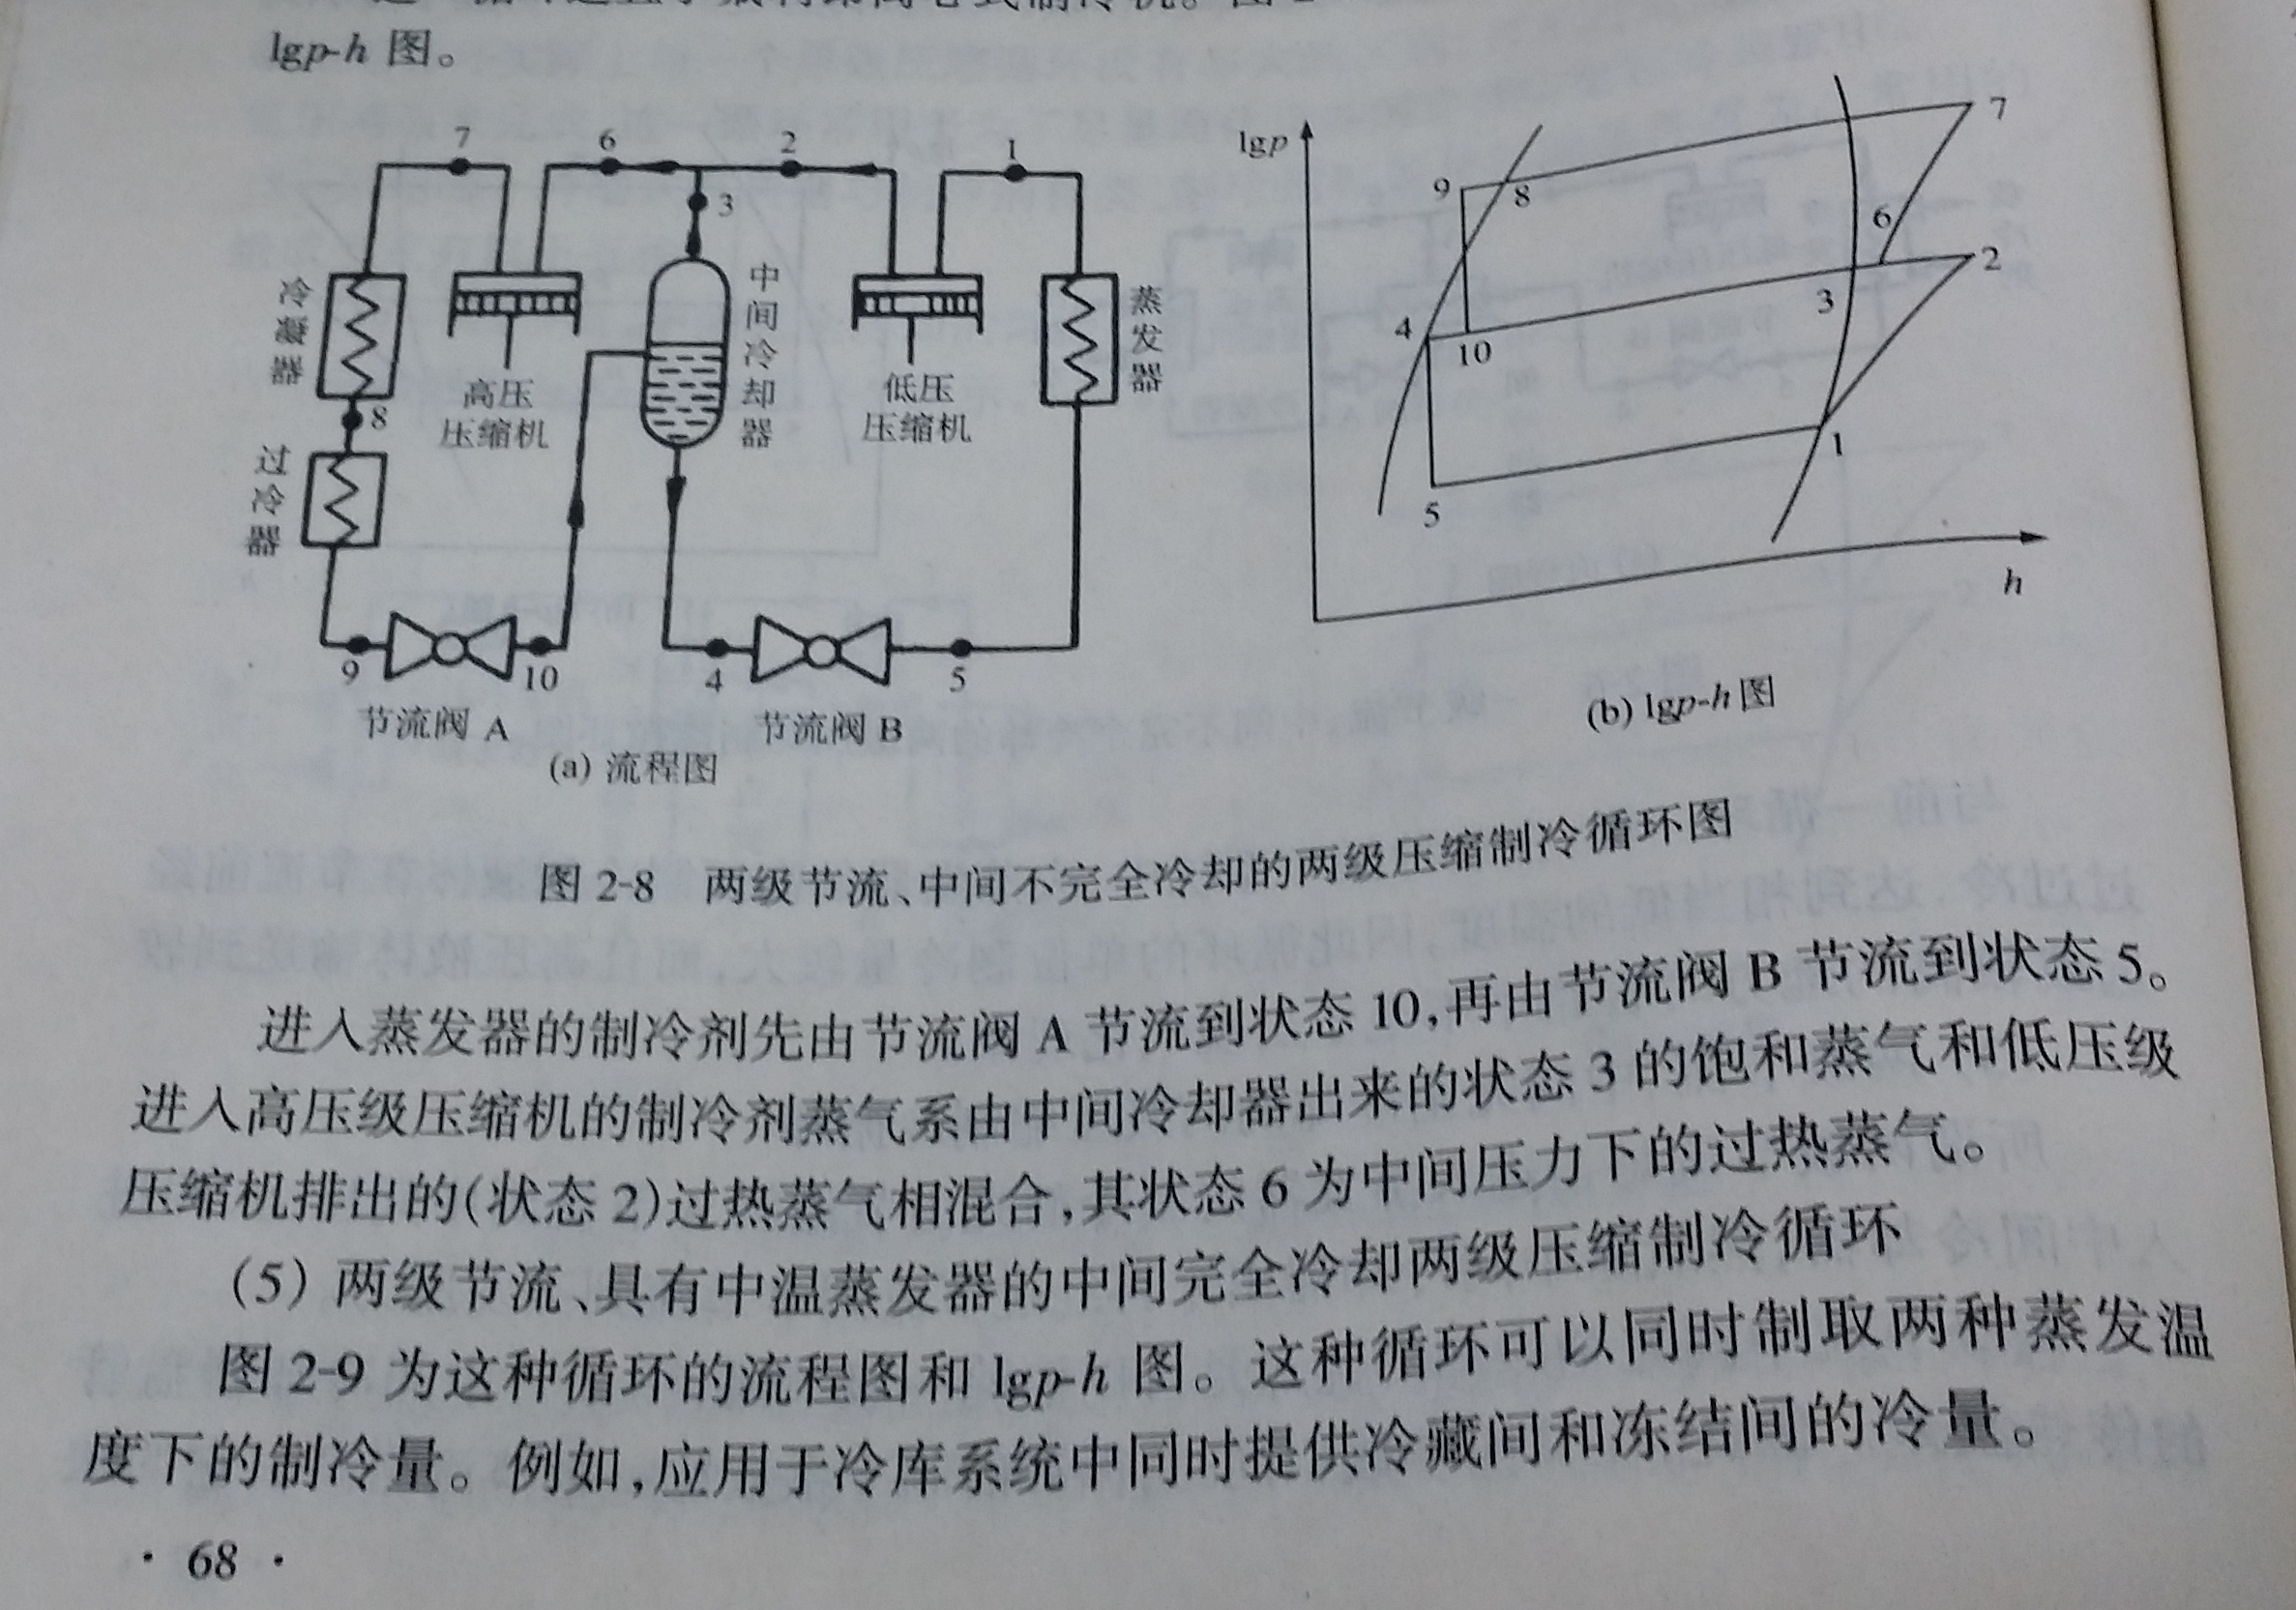
\includegraphics[width=\textwidth]{no51} 
	\caption{两级节流,中间不完全冷却双级压缩理论制冷循环的定义}
\end{figure}
\begin{figure}
	\begin{minipage}{0.45\textwidth}
		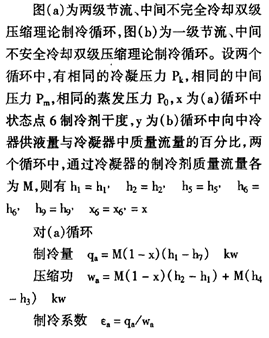
\includegraphics{no52}
	\end{minipage}
	\begin{minipage}{0.45\textwidth}
		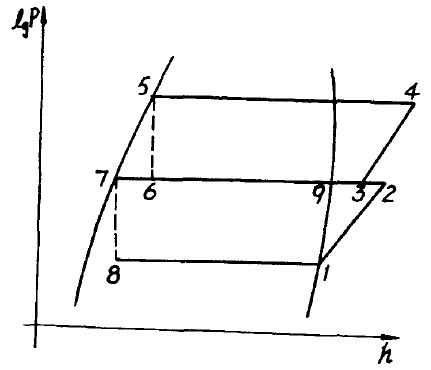
\includegraphics{no53}
	\end{minipage}
\caption{两级节流,中间不完全冷却双级压缩理论制冷循环的热力计算}
\end{figure}

\section{空压机、造水机二考一}
\textbf{造水机:}真空沸腾式海水淡化装置是基于盐几乎不溶于低压蒸汽的原理,首先用喷射泵对系统抽真空,一般要求真空度在90\%以上,用来制淡水的海水通过专用海水泵或辅海水泵旁通来供给,真空泵和排盐泵的工作水也由它来提供。海水经过截止止回阀进人竖管,竖管外壁充满温度较高的主机冷却水,海水在此
加温,当达到沸点后即开始汽化,蒸汽通过蒸馏器上方的管壳式冷凝器两侧的汽水分离器, 从冷凝器壳体上部开口进入。冷却用的海水在冷凝器管内流过,管外的蒸汽被冷凝为淡水,凝水聚集在冷凝器底部, 由凝水泵抽出送往制淡柜。 蒸发后剩下的高盐度海水由排盐泵排出,以保持造水机内部海水液位的平衡,再用海水对蒸汽进行冷凝,从而得到几乎不含盐的蒸馏水。抽真空的目的主要有以下两个方面:首先,由于水的沸点随着真空度的升高而降低,当真空度达到90\%时,海水沸腾的温度大概在$45℃$,而主机缸套水的出口温度一般控制在$80℃$,这样就可以用主机缸套水对海水进行加热,既使主机的废热得以利用,同时造水机又可以充当主机缸套水冷却器的作用,减少了主机缸套水冷却器的负荷,起到双重节能的作用,从而提高经济性。其次,由于蒸发温度低,则蒸发器表面不易结垢,尤其是硬质水垢的生成,使得维护保养工作较为容易。 

\textbf{空压机:}螺杆式空气压缩机的工作过程分为吸气、密封及输送、压缩、排气四个过程。当螺杆在壳体内转动时,螺杆与壳体的齿沟相互啮合,空气由进气口吸入,同时也吸入机油,由于齿沟啮合面转动将吸入的油气密封并向排气口输送;在输送过程中齿沟啮合间隙逐渐变小,油气受到压缩;当齿沟啮合面旋转至壳体排气口时,较高压力的油气混合气体排出机体。     采用变频器可通过改变螺杆转子转速的方式来改变排气量,当用气量发生变化时,变频器改变转速的方式调节空压机的排气量,达到排气压力恒定不变,并节约能源的目的。
\end{document}
